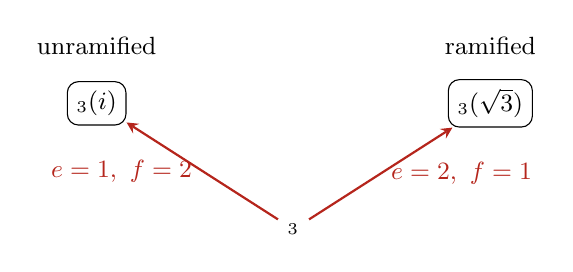
\begin{tikzpicture}[>=stealth,font=\small]
\node (a) at (0,0) {$\Q_3$};
\node[draw,rounded corners] (b) at (-2.5,1.6) {$\Q_3(i)$};
\node[draw,rounded corners] (c) at (2.5,1.6) {$\Q_3(\sqrt3)$};
\draw[->,BrickRed,thick] (a)--node[left] {$e=1,\ f=2$}(b);
\draw[->,BrickRed,thick] (a)--node[right] {$e=2,\ f=1$}(c);
\node[above] at (-2.5,2.1) {unramified};
\node[above] at (2.5,2.1) {ramified};
\end{tikzpicture}
